% \input{"//iab.baintern.de/Dfs/017/Ablagen/D01700-Info-Board/06_WMK/Corporate Design/Folienvorlagen/TeX-Folienformat.tex"}
\input{"/Users/jonathanlatner/Google Drive/My Drive/IAB/latex/TeX-Folienformat.tex"}


\documentclass[t,8pt,utfx8]{beamer}
\usepackage{booktabs}
\usepackage{setspace}
\usepackage{parskip}
\setbeamertemplate{caption}[numbered]
\newcommand{\sprache}{\englisch}
\renewcommand{\thesubsection}{\alph{subsection})}

\newcommand{\btVFill}{\vskip0pt plus 1filll}

\title[Balancing data utility and privacy]{Balancing data utility and privacy: Evaluating computer science and statistical approaches to creating synthetic data}
\subtitle{Statistische Woche\\
        Dortmund, Deutschland \\
         11. September, 2023}

\author{Jonathan Latner, PhD \newline Prof. Dr. Jörg Drechsler}

\newcounter{noauthorlines}
\setcounter{noauthorlines}{2} % Wert für 2 Autoren über 2 Zeilen. Ggf. anpassen

% %%%%%%%%%%%%%%
% Ende Anpassung
% %%%%%%%%%%%%%%

% \input{"//iab.baintern.de/Dfs/017/Ablagen/D01700-Info-Board/06_WMK/Corporate Design/Folienvorlagen/TeX-Folienformatierung_CD_2019"}
\input{"/Users/jonathanlatner/Google Drive/My Drive/IAB/latex/TeX-Folienformatierung_CD_2019"}

% Modify the section in toc template to enumerate
\setbeamertemplate{section in toc}{%
    \inserttocsectionnumber.~\inserttocsection\par
}

% use for subsections
\setbeamertemplate{subsection in toc}{}
% \setbeamertemplate{subsection in toc}{%
%     \setlength{\parskip}{1mm}
%     %     \hskip2mm -- \hskip1mm\inserttocsubsection\par
% }

\titlegraphic{\includegraphics[width=2cm]{/Users/jonathanlatner/Google Drive/My Drive/IAB/latex/CD 2019/aniged.png}}

\begin{document}


\section{Introduction}\label{sec_intro}
\frame[plain]{\titlepage}

\begin{spacing}{1.25}

%Table of contents
\begin{frame}
\frametitle{Sections}
\vskip6mm
\setlength{\leftskip}{0.5mm}
\setlength{\parskip}{5mm}
\begin{NoHyper}
        \tableofcontents
\end{NoHyper}
\end{frame}

\frame[c]{\frametitle{}
\centering
Section \ref{sec_intro}: Introduction
}



\frame{\frametitle{Overview}
\begin{itemize}
    \item {\bf Definition:} Synthetic data are data that mimic the characteristics of original or `real' data.
    \item {\bf Goal:} High utility + privacy protection = more knowledge
    \begin{itemize}
        \item Utility: any analysis using synthetic data should provide approximately the same answers as analysis using the original data.
        \item Privacy: Synthetic data look like real data, but without any of the threats to privacy contained in real data (theoretically).
        \item More knowledge is created if more data can be released with no (or little) risk to privacy, and accessed more easily.
    \end{itemize}
    \item {\bf The problem:} Trade off between utility and privacy 
    \item Different approaches for the generation of synthetic data have been developed.
    \begin{itemize}
        \item In statistics: formal guarantee of statistical utility, but no formal guarantee for privacy
        \item In computer science: formal guarantee of privacy, but no guarantee for statistical utility
    \end{itemize}
\end{itemize}
}

\frame{\frametitle{The goal}
\begin{itemize}
    \item Evaluate (compare and contrast) how different approaches to the creation of synthetic data balance the twin goals of data utility and data privacy.
    \item For now, we focus on utility (next steps: privacy)  
    \item In this talk, we will present some first results from this project.
\end{itemize}
}

\frame{\frametitle{Literature review}
\vskip -2mm
\begin{itemize}
    \item Not many papers that compare and contrast
    \item Most papers are often written by the package authors
    \begin{itemize}
                \item In these papers, their package is often the `winner'
        \item May be biased, but not necessarily wrong
        \item Different data packages solve different data problems
        \item Different data packages have different strengths and weaknesses
    \end{itemize}
    \item Few `independent' papers
    \begin{itemize}
                \item Little et al., 2021/2023 ({\emph Working paper})
        \begin{itemize}
            \item They don't tune the packages (defined later)
            \item Low data dimensionality/majority categorical data 
        \end{itemize}
        \item Dankar and Ibrahim (2021)
        \begin{itemize}
            \item 15 data sets (categorical, continuous, mixed)
            \item Low data dimensionality
            \item Only one measure of utility:  Prediction accuracy
        \end{itemize}
    \end{itemize}
\end{itemize}
}

\frame{\frametitle{Preview results}
\begin{itemize}
    \item 3 data packages (CTGAN, Datasynthesizer, Synthpop)
    \item 3 types of data
    \item Focus on utility (next step: privacy)
    \item Synthpop is the `winner' (similar to both Little et al., 2021/2023 and Dankar and Ibrahim, 2021)
    \item Our goal in the project is not only utility, but also to balance utility and privacy
    \item Adjusting the data dimensions (next steps)
\end{itemize}
}

\section{Data}\label{sec_data}
\frame[c]{\frametitle{}
\centering
Section \ref{sec_data}: Data
}

% \frame{\frametitle{Data}
% \begin{itemize}
%     \item 2 simulated data sets
%     \begin{itemize}
%         \item Using a `controlled' environment 
%         \item Isolate differences between synthetic data packages (tuning) and data structure (size, correlation, type, etc.)
%     \end{itemize}
%     \item 1  `real' data set
%     \begin{itemize}
%         \item Benchmark our results to published papers using these data
%     \end{itemize}
%     \item Others (next steps)
% \end{itemize}
% }

\frame{\frametitle{3 data sets}
\begin{itemize}
    \item 2 Simulated data sets - Examine differences in a controlled environment
    \begin{enumerate}
        \item Simulated categorical data 
        \begin{itemize}
            \item 1.000 observations
            \item 4 bivariate categorical variables (`Y', `N')
        \end{itemize}
        \item Simulated continuous data
        \begin{itemize}
            \item 1.000 observations
            \item 3 continuous variables (`income', `wealth', `age')
        \end{itemize}
    \end{enumerate}
    \item 1 Real data set
    \begin{itemize}
        \item UK 1991: Individual Sample of Anonymised Records (SAR) for the British Census, subsetted on the region of West Midlands
        \item 20\% sample ($\approx 20.000$)
        \item 12 variables: 1 numerical and 11 categorical, includes missing values
        \item Benchmark our results to Little et al., 2021/2023: 
    \end{itemize}
\end{itemize}
}


\section{Methods}\label{sec_methods}
\frame[c]{\frametitle{}
\centering
Section \ref{sec_methods}: Methods
}

\frame{\frametitle{Compare 3 packages for creating synthetic data}
\begin{itemize}
    \item We choose these three because they are commonly compared (Little et al., 2021/2023; Dankar and Ibrahim, 2021)
    \begin{enumerate}
        \item CTGAN (Conditional Tabular Generative Adversarial Network) in Synthetic Data Vault (SDV) package  (Patki et al., 2016)
        \item Datasynthesizer (Ping et al., 2017)
        \item Synthpop (Nowak et al., 2016)
    \end{enumerate}
\end{itemize}
\begin{table}[h]
\caption{Comparison of data synthesis packages}
\label{table_comparison}
\centering
\vskip -2mm
\begin{tabular}{lccc}
\toprule
Variable/data & CTGAN (GANs) & Datasynthesizer (PrivBayes) & Synthpop (CART) \\
\midrule
Continuous variables & & & \checkmark\\
Categorical variables & & & \checkmark \\
Mixed data & & & \checkmark \\
Privacy protection & \checkmark$^*$ & \checkmark & \\
High dimensional datasets & \checkmark & \checkmark & \\
\bottomrule
\multicolumn{4}{p{12cm}} {\footnotesize $^*$ In theory, GANs (Synthpop) offer no formal privacy protection.  In reality, one can adjust the training procedure of the discriminator to satisfy a formal guarantee (Beaulieu-Jones, et al., 2019; Neunhoffer, et al., 2021).}
\end{tabular}
\end{table}

}



\section{Tuning}\label{sec_tuning}
\frame[c]{\frametitle{}
\centering
Section \ref{sec_tuning}: Tuning
}

\frame{\frametitle{What is tuning?}
\begin{itemize}
    \item {\bf Definition:}  Adjusting the synthesis process to make the synthetic data more representative of the original data
    \item All data packages can be tuned to various levels
    \item All authors of data packages state that tuning the packages are important
    \item One should not simply use the default values
    \item Tuning is a time consuming process
    \item Not 100\% clear on how to best tune the data because
    \begin{itemize}
        \item No one, single measure for utility
        \item No one, single measure for privacy protection
    \end{itemize}
\end{itemize}
}

\frame{\frametitle{CTGAN (SDV)}
\begin{itemize}
    \item A total of 11 hyperparameters can be tuned, we focus on 4$^*$
    \begin{itemize}
        \item {\bf epochs} (3: 300, 600, 900): the number of iterations that the model will perform to optimize its parameters. Default is 300.  
        \item {\bf discriminator\_steps} (3: 1, 5, 10): Number of discriminator updates to do for each generator update. Default is 1.
        \item {\bf batch\_size} (2: 500, 1000): as well as the number of samples used in each step. Default is 500.  
        \item {\bf log\_frequency} (2: True, False): Whether to use log frequency of categorical levels in conditional sampling. It defaults to True. This argument affects how the model processes the frequencies of the categorical values that are used to condition the rest of the values. In some cases, changing it to False could lead to better performance.
    \end{itemize}
    \item copies (3: 1, 5, 10): Number of synthetic data sets
    \item Total: 576 synthetic data sets $\rightarrow$ 108 combinations of tuning parameters
\end{itemize}

\btVFill
\tiny

Source: \url{https://sdv.dev/SDV/user_guides/single_table/ctgan.html\#advanced-usage} \\
\url{https://docs.sdv.dev/sdv/single-table-data/modeling/synthesizers/ctgansynthesizer} \\
$^*$We don't use `discriminator\_dim', `discriminator\_decay', `discriminator\_lr', `embedding\_dim', `generator\_decay', `generator\_dim', `generator\_lr', `pac'


}

\frame{\frametitle{Datasynthesizer (PrivBayes)}
\begin{itemize}
    \item A total of 11 hyperparameters can be tuned, but we focus on 2$^*$
    \begin{enumerate}
        \item {\bf k} (3: 0, 1, 2).  The maximum number of parents in Bayesian network, i.e., the maximum number of incoming edges.  Default is 0.
        \item {\bf $\epsilon$} (7: 0, 0.1, 1, 5, 10, 20, 30).  Differential privacy. It roughly means that removing a row in the input dataset will not change the probability of getting the same output more than a multiplicative difference of exp($\epsilon$).  Set $\epsilon$=0 to turn off differential privacy.  Default is 0.1.  Epsilon value usually are less than one, but it’s not uncommon to see larger $\epsilon$ being used (i.e. U.S. Census is 19.61).$^\dagger$
    \end{enumerate}
    \item copies (3: 1, 5, 10): Number of synthetic data sets
    \item Total: 336 synthetic data sets $\rightarrow$ 63 combinations of tuning parameters
\end{itemize}

\btVFill
\tiny

Source: \url{https://github.com/DataResponsibly/DataSynthesizer/blob/master/DataSynthesizer/DataDescriber.py} \\
$^*$ Others available, but relate to dictionaries (`category\_threshold', `null\_values', `attr\_to\_datatype', `attr\_to\_is\_categorical', `attr\_to\_is\_candidate\_key', etc.) \\
$^\dagger$ \url{https://www.ncsl.org/health/differential-privacy-for-census-data-explained} 

}

\frame{\frametitle{Synthpop (CART)}
\begin{itemize}
    \item Many hyperparameters can be tuned, but we focus on 2$^*$
    \begin{enumerate}
        \item  {\bf complexity parameter} (5: 1e-8, 1e-6, 1e-4, 0.01).  A measure of the complexity of a tree.  Small values of cp will grow large trees, but this can also lead to overfitting.  Default is 0.00000001 (1e-8).
        \item {\bf minbucket} (4: 5, 10, 25, 50). the minimum number of observations in any terminal $<leaf>$ node. Default is 5.  
    \end{enumerate}
    \item copies (3: 1, 5, 10): Number of synthetic data sets
    \item Total: 256 synthetic data sets $\rightarrow$ 48 combinations of tuning parameters
\end{itemize}

\btVFill
\tiny

Source: \url[pg. 10-11]{https://cran.r-project.org/web/packages/synthpop/vignettes/utility.pdf} \\
\url{https://alfurka.github.io/2023-01-30-creating-synthetic-values-with-synthepop-cart/} \\
$^*$ Others available, but relate to dictionaries (minnumlevels, cont.na, etc.).  We don't use `proper' or `smoothing', at least not yet.


}

\section{Measuring utility}\label{sec_utility}
\frame[c]{\frametitle{}
\centering
Section \ref{sec_utility}: Measuring utility \\
}

\frame{\frametitle{Measuring utility}

\begin{itemize}
    \item Ratio of estimates (ROE)$^*$ 
    \begin{itemize}
        \item The average difference between the values (i.e. proportion/total) of a given categorical variable (or binned continuous variable) are between synthetic and original data
        \item Higher is better utility.  Max = 1, min = 0.  
        \item The ROE is calculated over univariate and  bivariate values of a given variable(s).  
    \end{itemize}
    \item Difference/overlap in the estimate/confidence interval$^\dagger$
    \begin{itemize}
        \item The average difference between each point estimate and confidence interval are from the same regression model applied to original and synthetic data
        \item Standardized difference (Std. Diff) - Lower is better utility (closer to 0).
        \item Confidence interval overlap (CIO) - Higher is better utility.  Max = 1, negative value indicating no overlap (here, negative = 0).
    \end{itemize}
    \item Others (next steps)
\end{itemize}
\btVFill
\tiny

$^*$ \url{https://github.com/clairelittle/psd2022-comparing-utility-risk/blob/main/code/ROC_Ratio_of_Counts_Estimates.R} \\
$^\dagger$ \url{https://github.com/clairelittle/psd2022-comparing-utility-risk/blob/main/code/CIO_Confidence_Interval_Overlap.R}

}

\frame{\frametitle{Methods}

For each package (Datasynthesizer, CTGAN, Synthpop), for each categorical hyperparameters ($h$), estimate the effect of each value ($j$) on each utility measure ($y_i$) (ROE\_u, ROE\_b, Std. Diff, and CIO) in model \ref{model_1} and for each set of copies ($m$) in model  \ref{model_2}.

\begin{align}
    y_i &= \beta_0 + \sum_{h=1}^{H}\sum_{j=1}^{J} \beta_{h,j} x_{h,j,i} + \epsilon \label{model_1}\\ 
    y_i &= \beta_0 + \sum_{h=1}^{H}\sum_{j=1}^{J} \beta_{h,j} x_{h,j,i} + \epsilon \in m=1,5,10 \label{model_2}
\end{align}

For example:
\begin{itemize}
    \item CTGAN has 4 hyperparameters ($h$) or 5 with copies ($m$), each of which have varying values ($j$).  
    \item One hyperparameter is epochs ($h$) and epochs have 3 values ($j$), 300, 600 or 900.  
\end{itemize}


}

\section{Results}\label{sec_results}
\subsection{Simulated categorical data}\label{sec_results_categorical}
\frame[c]{\frametitle{}
\centering
Section \ref{sec_results}: Results \\
Section \ref{sec_results}\ref{sec_results_categorical}: Simulated categorical data
}

\frame{\frametitle{Descriptive statistics - categorical data}
\vspace{-5mm}
\begin{figure}
    \caption{}
    \resizebox{\textwidth}{!}{\includegraphics{../../simulation_data/categorical/graphs/graph_descriptives.pdf}}
    \label{graph_descriptives_categorical}
\end{figure}
}


\frame{\frametitle{Measuring utility in CTGAN}
\vspace{-5mm}
\begin{figure}
    \caption{Sorted by Std. Diff}
    \resizebox{\textwidth}{!}{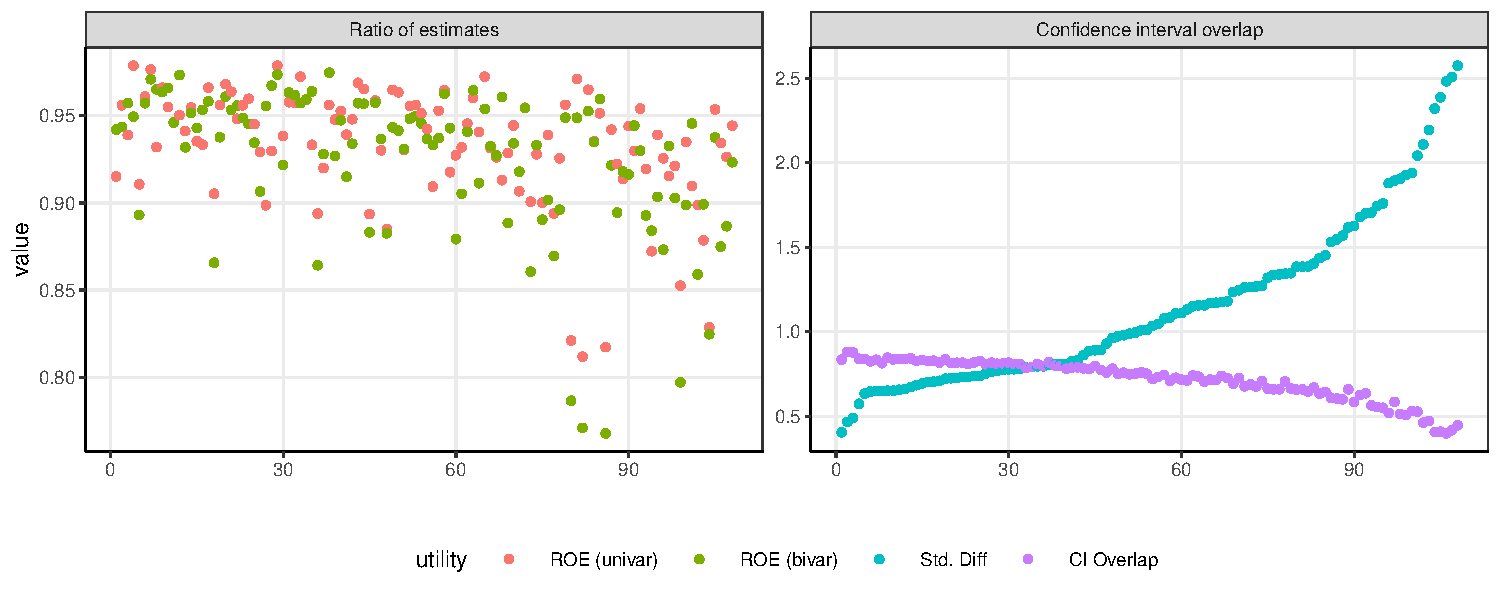
\includegraphics{../../simulation_data/categorical/graphs/ctgan/graph_compare_ctgan_utility.pdf}}
    \label{graph_compare_utility_sim_categorical_ctgan}
\end{figure}
}

\frame{\frametitle{Estimating utility in CTGAN (model \ref{model_1})}
\vspace{-5mm}
\begin{figure}
    \caption{Parametric estimates from linear model}
    \vspace{-5mm}
    \resizebox{\textwidth}{!}{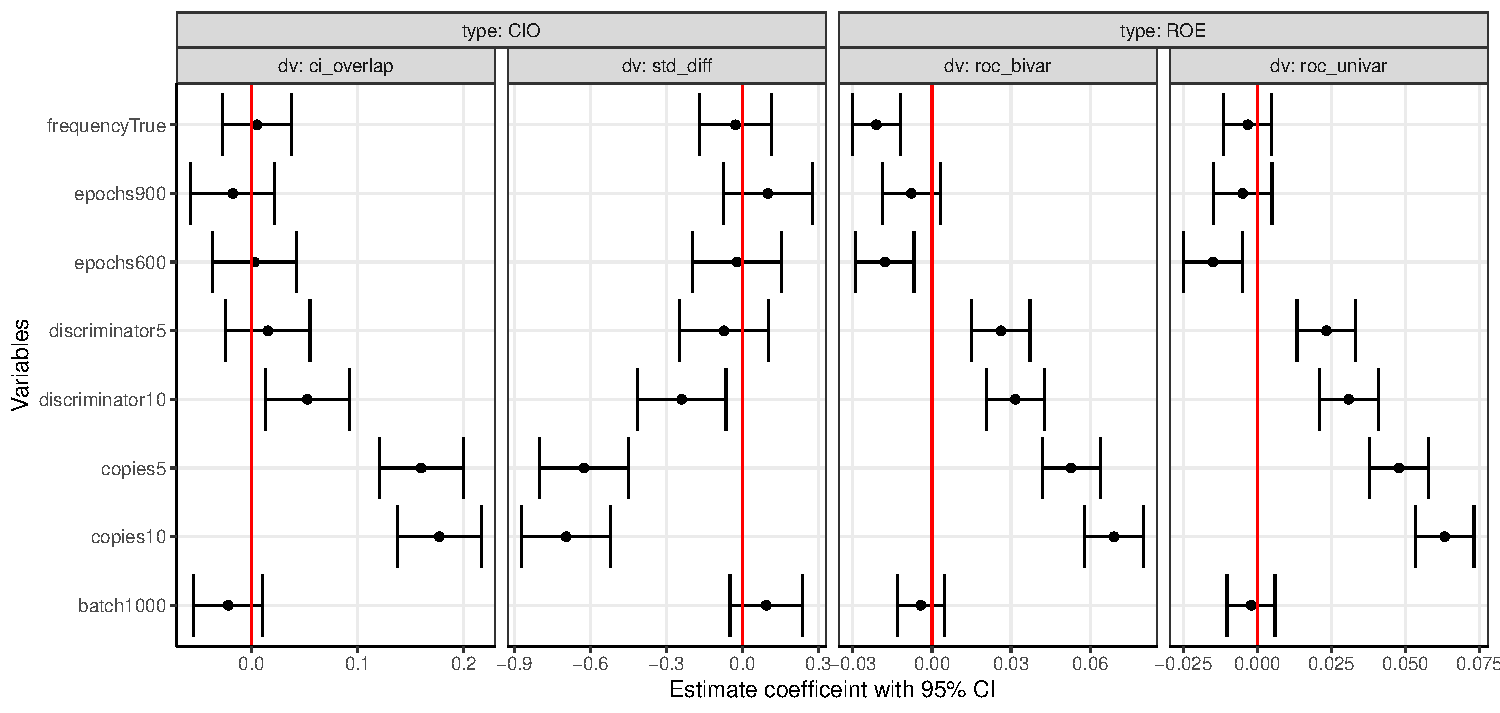
\includegraphics{../../simulation_data/categorical/graphs/ctgan/graph_ctgan_utility_compare.pdf}}
    \label{graph_ctgan_utility_compare}
\end{figure}
}

\frame{\frametitle{Estimating utility in CTGAN by copies ($m$)  (model \ref{model_2})}
\vspace{-5mm}
\begin{figure}
    \caption{Parametric estimates from linear model}
    \vspace{-5mm}
    \resizebox{\textwidth}{!}{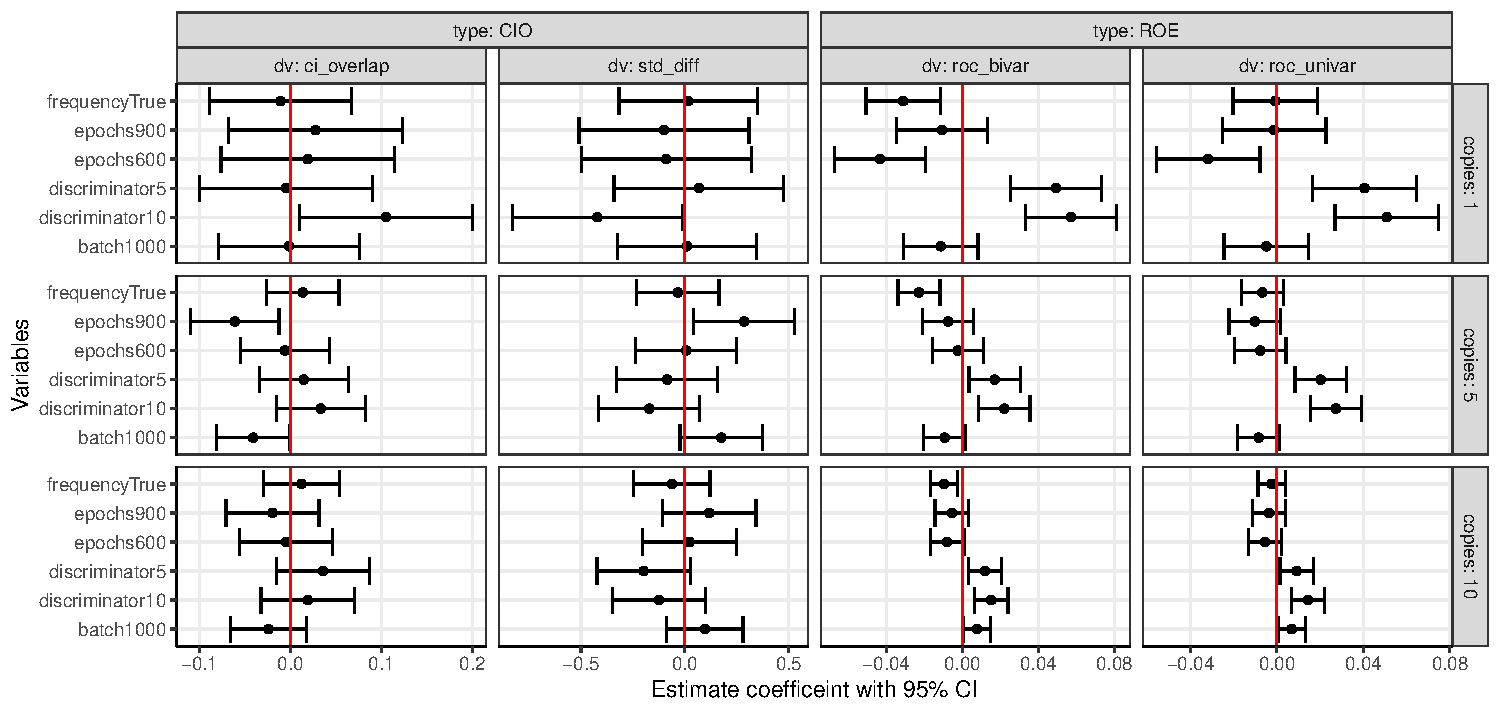
\includegraphics{../../simulation_data/categorical/graphs/ctgan/graph_ctgan_utility_compare_copies.pdf}}
    \label{graph_ctgan_utility_compare_copies}
\end{figure}
}


\frame{\frametitle{Compare frequency counts between baseline and tuned}
\vspace{-5mm}
\begin{figure}
    \caption{}
    \resizebox{\textwidth}{!}{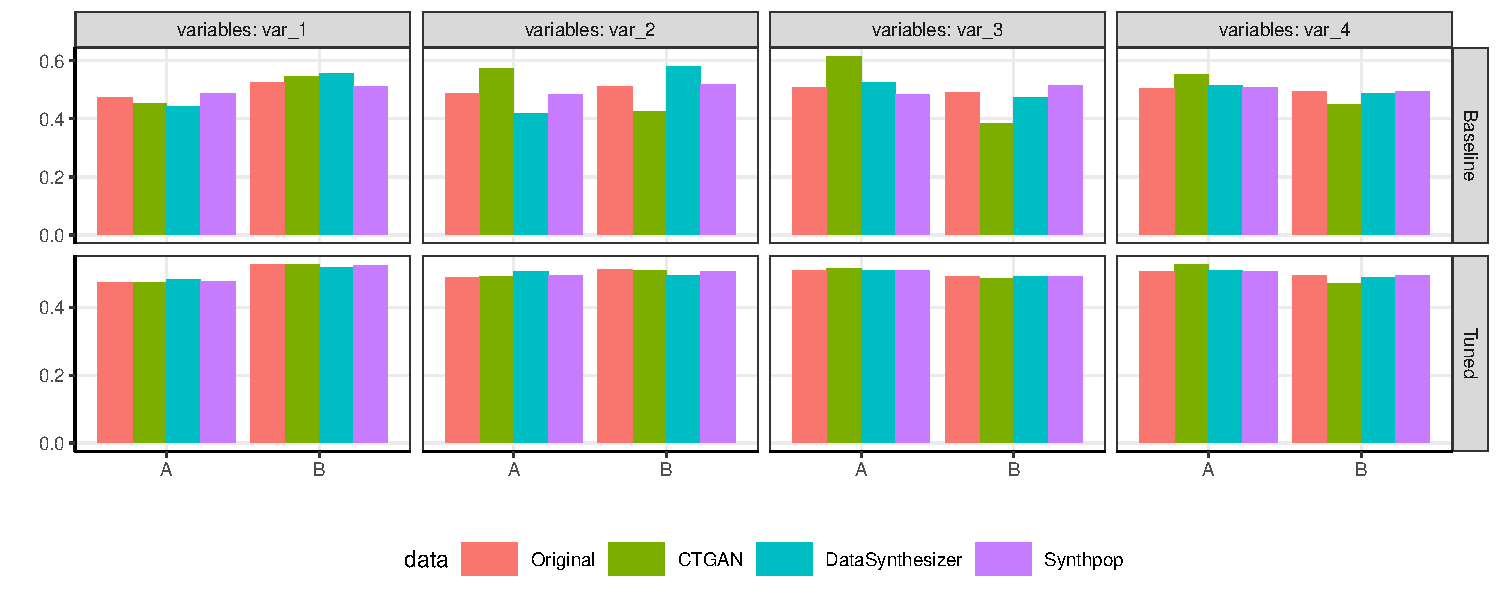
\includegraphics{../../simulation_data/categorical/graphs/graph_compare_frequency.pdf}}
    \label{graph_compare_frequency_categorical}
\end{figure}
}

\frame{\frametitle{Compare regression output between baseline and tuned}
\vspace{-5mm}
\begin{figure}
    \caption{}
    \resizebox{\textwidth}{!}{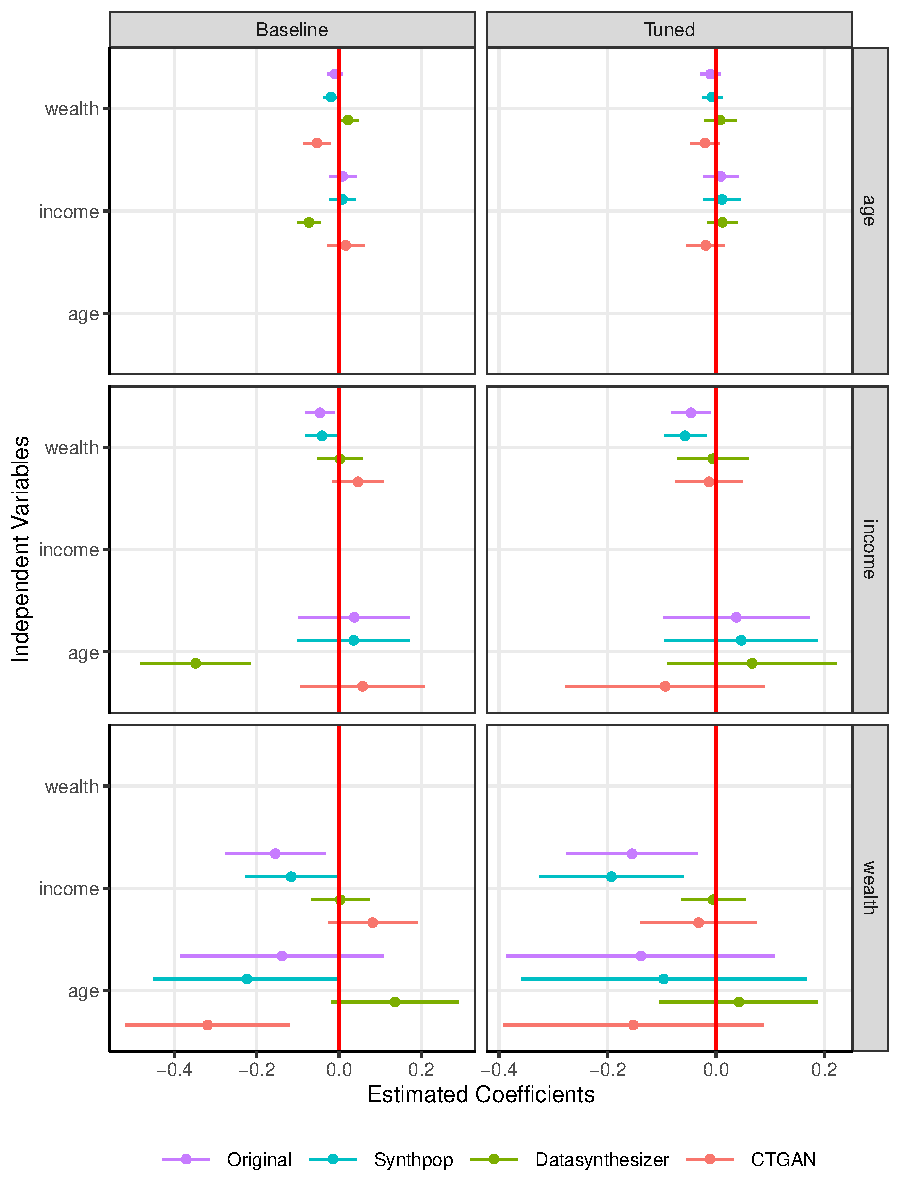
\includegraphics{../../simulation_data/categorical/graphs/graph_compare_cio_regressions.pdf}}
    \label{graph_compare_cio_regressions_categorical}
\end{figure}
}


\frame{\frametitle{Measuring utility for simulated categorical data}
\vspace{-5mm}
\begin{figure}
    \caption{}
    \resizebox{\textwidth}{!}{\includegraphics{../../simulation_data/categorical/graphs/graph_compare_utility.pdf}}
    \label{graph_compare_utility_sim_categorical}
\end{figure}
}

\frame{\frametitle{Summary: Synthpop has highest utility}
\begin{table}[h]
\caption{Comparison of Results}
\label{table_comparison}
\centering
\begin{tabular}{lrrrr}
\toprule
Data                            & ROE univar & ROE bivar & Std. Diff & CIO \\
\midrule
Simulated categorical variables & =          & =         & SP        & SP \\
\bottomrule
\end{tabular}
\end{table}
\begin{itemize}
    \item CTGAN/Datasynthesizer requires tuning (not Synthpop)
    \item Unexpectedly, CTGAN performs 2nd best for categorical data
\end{itemize}
}


\subsection{Simulated continuous data}\label{sec_results_continuous}
\frame[c]{\frametitle{}
\centering
Section \ref{sec_results}: Results \\
Section \ref{sec_results}\ref{sec_results_continuous}: Simulated continuous data
}

\frame{\frametitle{Descriptive statistics - continuous variables}
\begin{table}[!h]
    \caption{}
    \centering
    \resizebox{\textwidth}{!}{\begin{tabular}{rlrrrrr}
\toprule
number & variable & min & max & mean & std & median \\
\midrule
1 & age & 16.00 & 94.00 & 55.65 & 22.56 & 57.00 \\
2 & income & 624.00 & 349355.00 & 35721.10 & 41455.86 & 22421.50 \\
3 & wealth & -19560.00 & 89975356.00 & 659520.71 & 3165853.95 & 127616.00 \\
\bottomrule
\end{tabular}
}
    \label{table_variables_continuous}
\end{table}
}

\frame{\frametitle{Measuring utility for simulated continuous data}
\vspace{-5mm}
\begin{figure}
    \caption{}
    \resizebox{\textwidth}{!}{\includegraphics{../../simulation_data/continuous/graphs/graph_compare_utility.pdf}}
    \label{graph_compare_utility_sim_continuous}
\end{figure}
}

\frame{\frametitle{Summary: Synthpop has highest levels of utility}
\begin{table}[h]
\caption{Comparison of Results}
\label{table_comparison}
\centering
\begin{tabular}{lrrrr}
\toprule
Data                            & ROE univar & ROE bivar & Std. Diff & CIO \\
\midrule
Simulated continuous variables  & SP         & =         & SP        & SP \\
\bottomrule
\end{tabular}
\end{table}
\begin{itemize}
    \item CTGAN has similar level of CIO but higher Std. Diff
\end{itemize}
}


\subsection{UK 1991}\label{sec_results_UK1991}
\frame[c]{\frametitle{}
\centering
Section \ref{sec_results}: Results \\
Section \ref{sec_results}\ref{sec_results_UK1991}: Individual Sample of Anonymised Records (SAR) for the British Census, subsetted on the region of West Midlands (UK 1991)
}

\frame{\frametitle{Descriptive statistics - UK 1991}
\vspace{-5mm}
\begin{figure}
    \caption{}
    \vspace{-5mm}
    \resizebox{\textwidth}{!}{\includegraphics{../../UK1991/graphs/graph_descriptives.pdf}}
    \label{graph_descriptives}
\end{figure}
}

\frame{\frametitle{Measuring utility}
\vspace{-5mm}
\begin{figure}
    \caption{Ratio of estimates}
    \resizebox{\textwidth}{!}{\includegraphics{../../UK1991/graphs/graph_compare_utility_roe.pdf}}
    \label{graph_compare_utility_roe}
\end{figure}
}

\frame{\frametitle{Measuring utility}
\vspace{-5mm}
\begin{figure}
    \caption{Confidence interval overlap}
\vspace{-5mm}
    \resizebox{\textwidth}{!}{\includegraphics{../../UK1991/graphs/graph_compare_utility_cio.pdf}}
    \label{graph_compare_utility_cio}
\end{figure}
}

\frame{\frametitle{Comparing duration to create 1 synthetic data set ($\times5$)}
\begin{table}[!h]
    \caption{UK 1991 data, 12 variables (1 continuous), and  $\approx$ 20.000 observations}
    \centering
    \input{../../UK1991/tables/duration/table_duration.tex}
    \label{table_dution_UK1991}
\end{table}
}

\frame{\frametitle{Summary: things become more complicated in `real' data}
\begin{table}[h]
\caption{Comparison of Results}
\label{table_comparison}
\centering
\begin{tabular}{lrrrr}
\toprule
Data                            & ROE univar & ROE bivar & Std. Diff & CIO \\
\midrule
UK1991                          & DS/SP   & DS/SP        &           & \\
\hskip 5mm DV: MSTATUS          &            &           & CTGAN     & CTGAN \\
\hskip 5mm DV: TENURE           &            &           & SP        & SP \\
\bottomrule
\end{tabular}
\end{table}

}

\section{Conclusion}\label{sec_conclusion}
\frame[c]{\frametitle{}
\centering
Section \ref{sec_conclusion}: Conclusion
}

\frame{\frametitle{Summary}
\begin{table}[h]
\caption{Comparison of Results}
\label{table_comparison}
\centering
\begin{tabular}{lrrrr}
\toprule
Data                            & ROE univar & ROE bivar & Std. Diff & CIO \\
\midrule
Simulated categorical variables & =          & =         & SP        & SP \\
Simulated continuous variables  & SP         & =         & SP        & SP \\
UK1991                          & DS/SP   & DS/SP        &           & \\
\hskip 5mm DV: MSTATUS          &            &           & CTGAN     & CTGAN \\
\hskip 5mm DV: TENURE           &            &           & SP        & SP \\
\bottomrule
\end{tabular}
\end{table}
}



\frame{\frametitle{Results}
\begin{itemize}
    \item Main message: Synthpop is the `winner'
    \begin{itemize}
        \item However, it is not always the `best'
        \item Easy - little tuning required 
        \item Fastest
    \end{itemize}
    \item Datasynthesizer/CTGAN
    \begin{itemize}
        \item Requires tuning
    \end{itemize}
    \item CTGAN
    \begin{itemize}
        \item Slowest
    \end{itemize}
\end{itemize}
}

\frame{\frametitle{Next steps}
\begin{itemize}
    \item Results a reflection of low data dimensionality and focus on data utility
    \item Privacy protection
    \item High data dimensionality
\end{itemize}
}


\frame[c]{\frametitle{}
\centering
Thank you
}


\end{spacing}

\end{document}

